\documentclass[conference]{IEEEtran}
\usepackage{amsmath,amssymb,booktabs,array,enumitem,algorithm,algpseudocode,microtype,graphicx,pgfplots}
\usepackage[hidelinks]{hyperref}
\pgfplotsset{compat=1.18}
\usepgfplotslibrary{groupplots}
\providecommand*{\algorithmautorefname}{Algorithm}
\newcommand{\method}{SWT-CP}

\title{SWT-CP: Lightweight Trap-Based Free-Rider Mitigation in Federated Learning}
\author{\IEEEauthorblockN{Aashnan Rahman}
\IEEEauthorblockA{Department of Computer Science and Engineering\\
Islamic University of Technology\\Student ID: 231041006}}

\begin{document}
\maketitle

\begin{abstract}
\end{abstract}

\begin{IEEEkeywords}
federated learning, free riding, anomaly detection, robust statistics, client auditing, lightweight defense
\end{IEEEkeywords}

\section{Introduction}
Federated learning (FL) enables multiple clients to train a shared model without transferring their raw data to a central server. In a typical communication round, the server distributes the current global model, participating clients improve it using their local data, and the server aggregates their returned updates, for example through Federated Averaging (FedAvg) \cite{mcmahan2017communication}. This collaborative arrangement makes learning possible across distributed and privacy-sensitive data sources and has supported large-scale applications \cite{bonawitz2019towards,hard2018federated}.

The quality of the resulting global model nevertheless depends on clients actually performing the local work expected of them. In practice, some clients may decide not to contribute meaningful training. A client may have insufficient useful data, limited computation or energy, or may simply wish to conserve its own resources while continuing to receive the model produced by the federation. Such a participant is commonly described as a \emph{free rider} \cite{lin2019freeriders,fraboni2021freerider}. It obtains the benefit of the collaborative model while contributing little or no genuine learning in return.

Free riding differs from an active poisoning attack. A free rider does not necessarily attempt to insert a harmful objective, corrupt labels, or deliberately steer the global model in an adversarial direction. Its harmful effect is primarily an omission of useful work. Had the client trained honestly, its local data and computation could have produced an informative update and potentially improved the aggregated model. When it does not, the global model must depend more heavily on the remaining contributors. One inactive participant may have little visible effect, but widespread free riding reduces the effective training population, wastes communication and coordination resources, slows or weakens learning, and creates an unfair distribution of computational cost.

Accordingly, this work studies a lightweight server-side method for identifying clients that repeatedly avoid meaningful local training without relying on client-reported performance or resource information.

% The contributions of this work will be presented here as a bullet-point list.

\section{Related Work}
\subsection{Free-rider attacks}
Lin \emph{et al.} formalized free riding in FL and introduced both fabricated-update attacks and STD-DAGMM detection \cite{lin2019freeriders}. Fraboni \emph{et al.} showed that free riders can imitate successive global updates and disguise them with calibrated noise \cite{fraboni2021freerider}. Zhu \emph{et al.} subsequently constructed a stronger attack that matches geometric properties used by feature-based defenses \cite{zhu2023advanced}. Collectively, these works show that replay and arbitrary noise are insufficient evaluation targets: a detector based on a fixed, known update statistic can be imitated by a history-aware attacker.

\subsection{Statistical and Learning-Based Detection}
Statistical detectors use update norms, dispersion, cosine similarity, or temporal consistency because these signals are available at the server and relatively inexpensive. Their central weakness is that non-IID honest updates may also be outliers, while adaptive attackers can reproduce the statistics being monitored. \textbf{FRAD} improves on a single statistic by combining a DAGMM-style anomaly detector with contribution and reputation models \cite{wang2024frad}. \textbf{PASS} combines parameter auditing with contribution evaluation and considers both resource-poor and strategically selfish free riders \cite{wang2023pass}. Both enrich the evidence available to the server, but introduce auxiliary models or auditing assumptions, additional calibration, and greater computational cost. Their learned or engineered references may also require adaptation when the model architecture, data heterogeneity, or attacker behavior changes.

\subsection{Challenge-Based and Verifiable Computation}
\textbf{FRIDA} seeks evidence of genuine training through privacy-attack techniques \cite{recasens2024frida}. Its membership-inference variants use a shared canary batch, while its property-inference variants test whether inferred client-data properties remain plausible across rounds. This targets the cause of free riding more directly than update geometry, but adds client or server computation, requires individual-update access, and exposes a known canary objective that a capable attacker can deliberately satisfy. Trusted hardware, remote attestation, and cryptographic proof can provide stronger execution guarantees, but require specialized support or substantial proof and communication overhead; they also complicate integration with secure aggregation \cite{bonawitz2017practical}. The remaining gap is a lightweight server-side method that creates unpredictable evidence without auxiliary detector training, trusted client reports, public canary data, or specialized hardware.

\section{Threat Model and Attacks}
There are $N$ attributable clients and a coordinating server. In round $t$, client $i$ receives $w^{\mathrm{send}}_{t,i}$ and returns $w^{\mathrm{ret}}_{t,i}$. The server derives
\begin{equation}
\Delta_{t,i}=w^{\mathrm{ret}}_{t,i}-w^{\mathrm{send}}_{t,i},\qquad
r_{t,i}=\lVert\Delta_{t,i}\rVert_2.
\end{equation}
For an audited client, $w^{\mathrm{send}}_{t,i}$ is a perturbed trap rather than the aggregating global model. Clients receive no trap indicator, and trap-derived updates are excluded from aggregation.

Attackers know only models previously sent to them. They do not know the audit schedule, group membership, anchor identities, thresholds, or ground-truth labels. Four increasingly informed behaviors are evaluated.

\medskip\noindent\textbf{FR1---Playback}
\begin{equation}
\widehat w_{t,i}=w^{\mathrm{send}}_{t-1,i}.
\end{equation}
The client stores the last model it received and submits that model in the next round without training. During its first round, when no previous model exists, it returns the current received model. This is the least expensive attack, but it responds to a new model using stale information and may also create an exact or near-exact send-back.

\medskip\noindent\textbf{FR2---Bounded Random Update}
\begin{equation}
\widehat w_{t,i}=w^{\mathrm{send}}_{t,i}+\epsilon,qquad
\epsilon_j\sim\mathcal U(-10^{-3},10^{-3}).
\end{equation}
FR2 avoids an exact send-back by adding an independently sampled bounded value to every floating-point coordinate. The response is nonzero and superficially update-like, but it contains no information from local data and has no memory of earlier rounds. It represents a client attempting to bypass simple equality or zero-norm checks at negligible computational cost.

\medskip\noindent\textbf{FR3---Historical Averaging}
\begin{equation}
\widehat w_{t,i}=\frac{1}{|\mathcal H_{t,i}|}
\sum_{w\in\mathcal H_{t,i}}w,qquad |\mathcal H_{t,i}|\leq5.
\end{equation}
The client maintains a rolling history $\mathcal H_{t,i}$ of up to five models received from the server, including the current one, and returns their element-wise mean. Averaging produces a smooth, history-dependent response without local optimization. Because the client is not told which models are traps, every trap enters the same history and can affect several later responses.

\medskip\noindent\textbf{FR4---Trajectory Imitation}
\begin{equation}
d_s=w^{\mathrm{send}}_{s,i}-w^{\mathrm{send}}_{s-1,i},\quad
\widehat w_{t,i}=w^{\mathrm{send}}_{t,i}+\bar d+\eta,
\end{equation}
where $\bar d$ is the mean of the latest five received-model differences and Gaussian $\eta$ is normalized to 10\% of $\lVert\bar d\rVert_2$. At cold start, the attacker uses a small Gaussian update. FR4 therefore attempts to imitate the direction and scale of recent global evolution, making it more plausible than memoryless noise. Nevertheless, it uses every received model indiscriminately, so an undisclosed trap also contaminates its trajectory estimate.

Collusion, partial honest training, on--off participation, and defense-aware adaptation are outside the evaluated scope.

\section{SWT-CP Methodology}
\noindent\textbf{Detection primitives.}
For floating tensor $k$, a trap is generated as
\begin{equation}
\tau_k=w_{t,k}+0.01\max(\sigma(w_{t,k}),10^{-4})\xi_k,
\qquad \xi_k\sim\mathcal N(0,I).
\end{equation}
The tensor-wise standard deviation makes the perturbation architecture- and scale-aware; the factor 0.01 keeps it small enough to remain trainable, while the $10^{-4}$ floor ensures that nearly constant tensors are still challenged. Responses are evaluated only against responses to the same trap. For reference norms $R$, SWT-CP computes median $m_r$, median absolute deviation $d_r$, and
\begin{equation}
z^{\mathrm{norm}}_{t,i}=\frac{r_{t,i}-m_r}{\max(d_r,0.05)}.
\end{equation}
The magnitude signal fires when $|z^{\mathrm{norm}}_{t,i}|>3$. The absolute value detects both unusually weak and unusually strong responses. The threshold of three robust scales is deliberately conservative, and the 0.05 MAD floor prevents a nearly identical reference set from turning harmless numerical variation into an extreme score. For floating layer $k$, a scale-free profile is
\begin{equation}
p_{t,i,k}=\frac{\lVert\Delta_{t,i,k}\rVert_2}
{\sum_j\lVert\Delta_{t,i,j}\rVert_2}.
\end{equation}
Distance from the coordinate-wise median profile is standardized by median/MAD with floor 0.01; the profile signal also fires above three robust scales. Its smaller floor reflects the fact that profile coordinates are normalized to sum to one. Using the same three-scale rule for both signals avoids attack-specific tuning. Either signal can initiate candidate confirmation, but ordinary statistical penalties require both, so an honest client with only unusual update size or only unusual layer allocation is not punished. A response norm below $10^{-6}$ is treated separately as an exact-send-back tolerance rather than a learned statistical threshold.

Each active client occupies one of three states: unflagged ($U$), candidate ($C$), or suspicious ($S$). Let $q_i$ denote its cumulative penalty, $n_i$ its current-episode probe count, and $f_i$ its joint-failure count. The detector then proceeds through the following phases.

\subsection{Phase I: Warm-Up}
For the first ten rounds, every client receives the ordinary global model. Ten rounds allow the initial global trajectory to stabilize and give history-based behavior a genuine model history before controlled probing begins. Nonzero population outliers are deliberately ignored because no controlled challenge has yet been issued. Only an exact or near-exact send-back is treated as evidence, adding five permanent points. Five is reserved for this strongest evidence so that three repeated send-backs reach the removal threshold of 15, while a single numerical accident cannot remove a client. This prevents natural early-training heterogeneity from populating the candidate set before the server has a trap-based reference. The procedure is summarized in \autoref{alg:warmup}.

\begin{algorithm}[t]
\caption{Phase I: warm-up}
\label{alg:warmup}
\begin{algorithmic}[1]
\Require global state $w_t$, active clients $V_t$
\ForAll{$i\in V_t$}
 \State send $w_t$ and receive $w^{\mathrm{ret}}_{t,i}$
 \State compute $\Delta_{t,i}$
 \If{$\lVert\Delta_{t,i}\rVert_2<10^{-6}$}
   \State $q_i\gets q_i+5$
 \EndIf
\EndFor
\State remove $i$ after three near-zero responses
\State aggregate all other ordinary responses with FedAvg
\end{algorithmic}
\end{algorithm}

\subsection{Phase II: Double Coverage}
The server shuffles the 100-client population into ten base groups, giving a nominal group size of ten without making group membership observable to clients. In each round it probes two groups, preserving approximately 80\% of clients for aggregation while completing one pass in five rounds. Two independently generated trap models, $\tau_A$ and $\tau_B$, are used in randomized passes; every client therefore responds once to each trap over ten rounds. Two challenges prevent a single favorable or unfavorable trap response from deciding initial suspicion. Evidence is stored until both passes finish, and responses to $\tau_A$ and $\tau_B$ are calibrated separately so different challenges do not share a reference distribution.

Two joint magnitude/profile failures can immediately move a client to $S$: repeat agreement across both independent traps is required for direct escalation. A weaker anomaly moves it to $C$ for fresh confirmation. Each joint coverage failure adds two points, an intermediate weight reflecting controlled but population-level evidence, while each near-zero response adds five. Every probed response is withheld from the global aggregation so deliberate trap updates cannot alter the production model. \autoref{alg:coverage} gives the complete sweep.

\begin{algorithm}[t]
\caption{Phase II: double coverage sweep}
\label{alg:coverage}
\begin{algorithmic}[1]
\Require active clients $V$, traps $\tau_A,\tau_B$
\State randomly partition $V$ into ten base groups
\ForAll{$\tau\in\{\tau_A,\tau_B\}$}
 \State randomize a five-round pairing of the ten groups
 \ForAll{paired groups $G$}
   \State send $\tau$ to every $i\in G$; store $\Delta_i$ and $p_i$
   \State exclude $G$ from the current aggregation
 \EndFor
 \State compute norm/profile references using only responses to $\tau$
\EndFor
\ForAll{$i\in V$}
 \State add two points per joint failure and five per near-zero response
 \If{two joint failures} \State move $i$ to $S$
 \ElsIf{either signal fires} \State move $i$ to $C$
 \EndIf
\EndFor
\end{algorithmic}
\end{algorithm}

\subsection{Phase III: Surveillance and Candidate Confirmation}
Clients remaining in $U$ are shuffled across ten surveillance groups. Retaining ten groups preserves the nominal ten-client comparison scale used during coverage. One group per round receives a shared surveillance trap; probing only one group preserves roughly 90\% of ordinary contributions, and after ten rounds every group has been observed once. The server then evaluates the completed sweep and starts another with a new trap. A joint surveillance failure carries only one point because it is the broadest and most heterogeneous comparison. Any statistical anomaly places a client in $C$, where it is withheld from aggregation and receives a fresh group-specific trap in subsequent rounds.

Each candidate group is paired with up to three rotating anchors that have never been flagged. Three permits a median reference to tolerate one atypical anchor, while a global cap of ten anchors limits the number of honest updates withheld when several candidate or suspicious groups coexist. Candidates and anchors receive the same trap, making the anchor distribution a local reference for that challenge. Two joint candidate failures confirm $S$, again requiring repeated fresh-trap evidence rather than one outlier. A candidate that produces a normal confirmation is returned to $U$ and its current magnitude episode is cleared so one false accusation does not bias later episodes. Off-duty anchors remain in ordinary surveillance and contribute normally. This rotating confirmation process appears in \autoref{alg:surveillance}.

\begin{algorithm}[t]
\caption{Phase III: surveillance and confirmation}
\label{alg:surveillance}
\begin{algorithmic}[1]
\State probe the next of ten $U$ groups with the sweep trap
\If{the surveillance sweep is complete}
 \State calibrate same-trap norm and profile statistics
 \State move anomalous clients $U\rightarrow C$
\EndIf
\ForAll{candidate groups $C_g$}
 \State rotate up to three never-flagged anchors $A_g$
 \State generate fresh trap $\tau_g$ and send it to $C_g\cup A_g$
 \State compare candidates with the same-trap anchor reference
 \If{candidate accumulates two joint confirmations}
   \State move candidate $C\rightarrow S$
 \ElsIf{candidate passes confirmation}
   \State return candidate $C\rightarrow U$ and clear episode evidence
 \EndIf
\EndFor
\State withhold surveillance, candidate, and anchor trap responses
\end{algorithmic}
\end{algorithm}

\subsection{Phase IV: Suspicion, Penalties, and Rehabilitation}
Suspicious clients are divided into approximately one group per ten suspects and are challenged every round. A ten-client target keeps groups large enough for future resistance to simple response sharing without imposing a hard maximum group size as $S$ shrinks. Each group receives its own fresh trap and rotating same-trap anchors. A joint suspicion failure adds three points because a same-trap, anchor-relative failure is stronger than population evidence; a near-zero response adds five. Statistical removal requires $q_i\geq15$ and at least ten suspicion probes. The threshold therefore needs five strong anchor-relative failures, or three exact send-backs, rather than one extreme observation. Ten probes also provide a meaningful denominator for rehabilitation. After that minimum, a client with $f_i/n_i\leq0.10$---at most one joint failure in ten probes---is instead rehabilitated: it returns to $U$ and its current magnitude penalty is cleared. This ``mercy'' rule prevents an initially false suspicion from keeping an otherwise consistent client under permanent intensive auditing. Near-zero penalties are permanent, so repeated exact send-backs cannot be erased through rehabilitation. The decision process is specified in \autoref{alg:suspicion}.

\begin{algorithm}[t]
\caption{Phase IV: weighted suspicion and decision}
\label{alg:suspicion}
\begin{algorithmic}[1]
\State form approximately $\max(1,\lfloor|S|/10\rfloor)$ suspect groups
\ForAll{suspect groups $S_g$}
 \State attach rotating anchors $A_g$ and generate fresh trap $\tau_g$
 \State send $\tau_g$ to $S_g\cup A_g$ and withhold all responses
 \ForAll{$i\in S_g$}
   \State $n_i\gets n_i+1$
   \If{joint failure} \State $q_i\gets q_i+3$; $f_i\gets f_i+1$
   \EndIf
   \If{near-zero response} \State add five permanent points
   \EndIf
   \If{$n_i\geq10$ and $f_i/n_i\leq0.10$}
     \State rehabilitate $i$ and clear magnitude-episode points
   \ElsIf{$n_i\geq10$ and $q_i\geq15$}
     \State remove $i$ from the federation
   \EndIf
 \EndFor
\EndFor
\State aggregate only active, non-trapped, non-candidate responses
\end{algorithmic}
\end{algorithm}

\medskip\noindent\textbf{Lightweight implementation.}
For a model with $P$ floating parameters and $L$ tensors, processing one returned model requires one parameter pass, $O(P)$ arithmetic, and an $L$-dimensional profile. Medians operate on scalar norms and short profiles; the server neither recomputes gradients nor trains a detector. Client software performs ordinary local training on whichever model it receives and does not train a second model. Apart from model/trap tensors, server state consists mainly of small per-client counters and bounded histories. Cost arises from probe training and temporary exclusion of trap responses, not an auxiliary learning pipeline.

\section{Experimental Design}
MNIST \cite{lecun1998gradient} and CIFAR-10 \cite{krizhevsky2009learning} are trained with convolutional models using 100 fully participating clients, 100 rounds, three local epochs, batch size 32, and SGD with learning rate 0.01 and momentum 0.9. Data are IID or allocated by a Dirichlet distribution with concentration $\alpha=0.5$. MNIST is evaluated with 30\% and 40\% free riders, while the available CIFAR-10 evaluation uses 40\% free riders.

Experiments are repeated under multiple random seeds. Seed identifiers and execution counts are omitted from the tables. For this preliminary capability summary, each attack is represented by its best observed completed result across the evaluated seeds; configuration-level metrics then combine the four selected attack results. Consequently, the tables report demonstrated best-observed performance rather than mean or worst-case reliability.

A positive prediction means permanent removal. We report $TP$, $FP$, $FN$, precision, recall, and $F1$. Unresolved candidates are reported separately because they are quarantined but not permanently removed. Accuracy, runtime, memory, state transitions, anchor composition, and trap assignments are also logged.

\section{Results}
\subsection{Best-Observed Multi-Seed Performance}
Table~\ref{tab:aggregate} places both datasets, both partitions, and both attacker shares in one grouped view. It summarizes the best observed result for each attack across multiple seeds and then combines FR1--FR4 within each available configuration. Recall reaches 100\% in every displayed configuration. MNIST precision ranges from 93.75\% to 100\%, whereas CIFAR-10 non-IID precision falls to 85.11\%, showing that heterogeneous data primarily increases false removal rather than missed detection in the selected results. CIFAR-10 30\% cells are marked as not evaluated because no corresponding experiments are available.

\begin{table*}[t]
\centering
\caption{Best observed multi-seed performance. Each available setting combines the strongest completed observation for each of FR1--FR4. A dash denotes a setting that was not evaluated.}
\label{tab:aggregate}
\setlength{\tabcolsep}{3.5pt}
\begin{tabular}{llrrrrrrrr}
\toprule
& & \multicolumn{4}{c}{30\% free riders} & \multicolumn{4}{c}{40\% free riders} \\
\cmidrule(lr){3-6}\cmidrule(lr){7-10}
Dataset & Partition & Precision & Recall & F1 & Accuracy & Precision & Recall & F1 & Accuracy \\
\midrule
MNIST & IID     & 99.17\% & 100\% & 99.59\% & 98.93\% & 100\%   & 100\% & 100\%   & 98.89\% \\
MNIST & Non-IID & 93.75\% & 100\% & 96.77\% & 98.90\% & 96.97\% & 100\% & 98.46\% & 98.89\% \\
CIFAR-10 & IID     & -- & -- & -- & -- & 100\%   & 100\% & 100\%   & 76.80\% \\
CIFAR-10 & Non-IID & -- & -- & -- & -- & 85.11\% & 100\% & 91.95\% & 74.48\% \\
\bottomrule
\end{tabular}
\end{table*}

\subsection{Detection Progress}
Figure~\ref{fig:detection-progress} reports cumulative permanent removals rather than temporary flags. The earliest removals occur at round 30, consistent with ten warm-up rounds, the ten-round double-coverage sweep, and the minimum ten suspicion probes required before statistical removal. In the selected IID results, all free riders are removed by round 30 on CIFAR-10 and by round 32 on MNIST. Non-IID 30\% MNIST also completes by round 32. The non-IID 40\% curves have longer FR4-driven tails: 90\% and 100\% removal occur by rounds 73 and 83 on MNIST, and by rounds 82 and 92 on CIFAR-10.

\begin{figure*}[t]
\centering
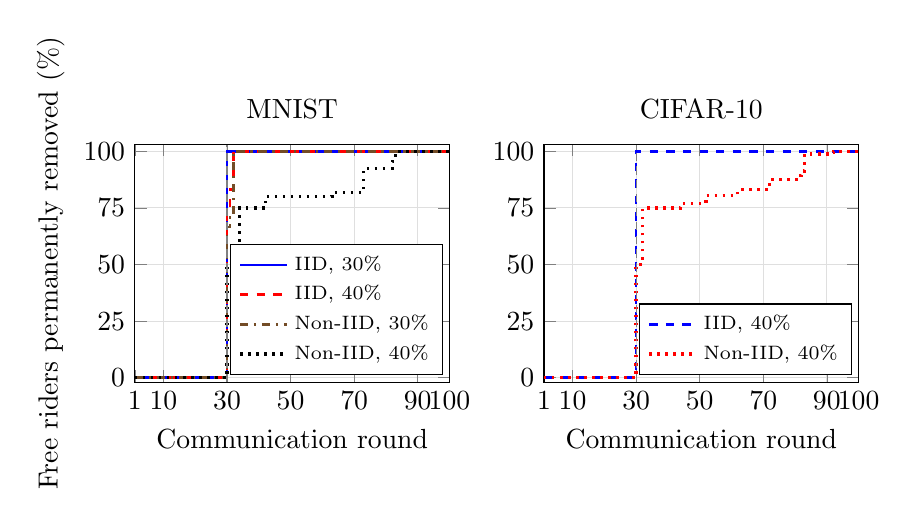
\begin{tikzpicture}
\begin{groupplot}[
 group style={group size=2 by 1, horizontal sep=1.2cm},
 width=0.46\textwidth,
 height=4.6cm,
 xmin=1, xmax=100,
 ymin=-2, ymax=103,
 xtick={1,10,30,50,70,90,100},
 ytick={0,25,50,75,100},
 xlabel={Communication round},
 grid=both,
 major grid style={draw=gray!25},
 no markers,
 every axis plot/.append style={line width=0.9pt},
 legend style={font=\scriptsize,at={(0.98,0.03)},anchor=south east},
 legend cell align={left}
]
\nextgroupplot[title={MNIST},ylabel={Free riders permanently removed (\%)}]
 \addplot+[const plot] coordinates {(1,0) (30,100) (100,100)};
 \addlegendentry{IID, 30\%}
 \addplot+[const plot,dashed] coordinates {(1,0) (30,75) (31,83.125) (32,100) (100,100)};
 \addlegendentry{IID, 40\%}
 \addplot+[const plot,dashdotted] coordinates {(1,0) (30,66.67) (31,71.67) (32,100) (100,100)};
 \addlegendentry{Non-IID, 30\%}
 \addplot+[const plot,dotted,line width=1.2pt] coordinates {(1,0) (30,50) (34,75) (42,80) (63,81.875) (73,92.5) (82,95.625) (83,100) (100,100)};
 \addlegendentry{Non-IID, 40\%}
 \draw[densely dashed,gray] (axis cs:30,-2) -- (axis cs:30,103);

\nextgroupplot[title={CIFAR-10}]
 \addplot+[const plot,dashed] coordinates {(1,0) (30,100) (100,100)};
 \addlegendentry{IID, 40\%}
 \addplot+[const plot,dotted,line width=1.2pt] coordinates {(1,0) (30,50) (32,75) (44,76.875) (52,80.625) (62,83.125) (72,87.5) (81,89.375) (82,91.25) (83,98.75) (91,99.375) (92,100) (100,100)};
 \addlegendentry{Non-IID, 40\%}
 \draw[densely dashed,gray] (axis cs:30,-2) -- (axis cs:30,103);
\end{groupplot}
\end{tikzpicture}
\caption{Cumulative permanent removal of free riders by communication round. Curves use the same best-observed per-attack selections as Table~\ref{tab:aggregate}; the vertical guide marks round 30, the earliest statistical-removal point under the configured schedule.}
\label{fig:detection-progress}
\end{figure*}

\subsection{Utility and execution cost}
Best-observed final accuracy is 98.89--98.93\% on MNIST and 74.48--76.80\% on CIFAR-10. Accuracy and detection remain distinct: a strong global model does not by itself establish that free riders were identified correctly.

Table~\ref{tab:cost} gives a deliberately compact execution profile. Values first average repeated seeds within each attack and then weight FR1--FR4 equally. Timings are descriptive rather than a controlled hardware benchmark: most configurations ran on CPU, while MNIST IID 40\% used CUDA. The device is therefore retained beside time per round, and peak memory is included as a direct lightweight-resource measure.

\begin{table}[t]
\centering
\caption{Recorded execution profile. Peak RSS is the mean of per-execution peaks.}
\label{tab:cost}
\footnotesize
\setlength{\tabcolsep}{2.5pt}
\begin{tabular}{llclrr}
\toprule
Dataset & Partition & Share & Device & s/round & RSS (GB) \\
\midrule
MNIST & IID     & 30\% & CPU  & 47.1 & 0.92 \\
MNIST & IID     & 40\% & CUDA & 55.6 & 1.40 \\
MNIST & Non-IID & 30\% & CPU  & 44.8 & 0.72 \\
MNIST & Non-IID & 40\% & CPU  & 43.6 & 0.84 \\
CIFAR-10 & IID     & 40\% & CPU & 88.9 & 1.85 \\
CIFAR-10 & Non-IID & 40\% & CPU & 79.5 & 1.90 \\
\bottomrule
\end{tabular}
\end{table}

Client simulations are serial, so these durations include local training rather than only detector overhead. Detection itself adds differencing, profile construction, robust scalar statistics, counters, and trap generation, but no auxiliary-model training.

\section{Discussion and Limitations}
The best-observed results show that SWT-CP can remove all four free-rider types under both IID and non-IID data. The principal remaining error is false removal under heterogeneous data, particularly on CIFAR-10, where honest update diversity weakens population and anchor-relative comparisons.

Because the present tables intentionally report the best observation across multiple seeds, they demonstrate capability but do not estimate average reliability or variance. A final evaluation should report all preregistered repetitions with uncertainty intervals and should separate partition, attacker, model, and trap randomness.

The study uses two image datasets, one non-IID concentration, full participation, and always-on non-colluding attackers. It does not test partial training, on--off behavior, defense-aware adaptation, dropout, or collusion. No external defense was rerun identically, so no comparative-superiority claim is made. Positive anchor qualification, repeated independent panels before candidate clearing, and paired within-client trap responses are priority extensions.

SWT-CP also requires attributable updates and temporarily spends honest computation on withheld responses. It is not directly compatible with ordinary secure aggregation \cite{bonawitz2017practical}; private deployment would require securely computed audit statistics or a separate challenge protocol.

\section{Conclusion}
SWT-CP shows that secret server-generated traps and robust statistics can provide useful free-rider evidence without trusted client telemetry or a learned detector. Its best observed multi-seed results attain 100\% recall across FR1--FR4 on MNIST and CIFAR-10 under both IID and non-IID partitions. Precision remains high on MNIST and IID CIFAR-10 but declines under non-IID CIFAR-10, identifying heterogeneous honest updates as the next target for improving anchor qualification and calibration.

\bibliographystyle{IEEEtran}
\bibliography{refs}
\end{document}
